\chapter{Work description}
\label{cap:descripcionTrabajo}

We designed a simple structure to organize all the scripts. As we are implementing different versions of the engine, there are specific modules that are compulsory to have well distinguished and possibly selected between them. Those modules are presented in the following Section~\ref{sec:modules}.

\vspace{1em}

\noindent Next, the key point is how to represent each required structure, including the board, chess pieces, precomputed tables, transposition tables, etc., as discussed in Section~\ref{sec:code}.

\section{Modules}
\label{sec:modules}

Each module is responsible for a specific aspect of the chess engine's functionality. The good part about this modular design is that it ensures clarity, maintainability, and the ability to test and improve individual components independently even more so when it comes to development with more people.

\subsection{Board}

\noindent This module handles the representation of the chessboard, as previously mentioned in Section~\ref{sec:board}, and the state of the game. It includes:
\begin{itemize}
    \item Representation of the chessboard with its pieces using bitboards for efficiency.
    \item Functions to make and unmake moves, including special moves like castling and en passant.
    \item Updating game state variables, such as castling rights or the half-move counter.
\end{itemize}

\noindent This module is vital, as it provides the data structures and operations required by other modules.

\subsection{Evaluation}

This module returns the final evaluation, a positive, 0, or negative number, depending on the current position.

\subsubsection{Move Generator}

This module generates the list of legal moves generated depending on the board while updating relevant information such as king's danger masks, pinned pieces or checking pieces, and calculating each piece moves. All chess rules are taken into consideration.

\subsection{Move ordering}

This module uses a heuristic to return a prioritized list of moves to improve the efficiency of the search.

\subsection{Search}

This module must return a set of search results, each containing the best move and the achieved evaluation at a specific depth.

\subsection{UCI}

This module is responsible for processing commands to invoke each module, following UCI standards.

\section{Code implementation}
\label{sec:code}

Although the previous algorithms were presented in pseudocode, from this point onward, all code implementations will be written in C++.

\subsection{Data representation}

\subsubsection{Square}

There are 64 possible squares on a chessboard so the first thought is to use a 6-bit structure which seem like a perfect match ($2^6 = 64$). However, modern processors are optimized to work with data sizes aligned to multiples of 8 bits (1 byte). Then, using 6 bits would require packing the data into more complex structures, which could introduce additional overhead in terms of bit manipulation and memory access. We preferred clarity and performance over micro-optimizations that complicate readability so we used a \texttt{uint8\_t} to describe a square.

\vspace{1em}

\noindent Moreover, masks are extremely useful for efficiently identifying and manipulating the squares on a chessboard using bitwise operations. Some of these masks are defined as constants in the code and others are calculated during compilation time. For example, they can be used to identify the column of a square or simply placing a new piece on board.

\begin{lstlisting}[breaklines=true, frame=single, caption={Square class.}]
class Square {
    uint8_t sq_value;

    constexpr bool is_valid() const {
        return sq_value < 64U;
    }

    constexpr uint64_t mask() const {
        return is_valid() ? 1ULL << sq_value : 0ULL;
    }

    // Calculating the column of a square (sq_value % 8)
    constexpr int col() const {
        return is_valid() ? sq_value & 7U : COL_INVALID;
    }
}

// Placing a piece by setting the bit corresponding to the
// square to 1
const uint64_t mask = square.mask();
bitboard_all |= mask;
\end{lstlisting}

\noindent Just to clarify, \texttt{sq\_value} must be a value between $0$ and $63$, inclusive, for the 64 squares on a chessboard. To calculate the column of a square, an AND operation is applied: \texttt{sq\_value \& 7U} extracts the 3 least significant bits, which correspond to the column of the square. Columns are enumerated from $0$ (A) to $7$ (H).

\subsubsection{Piece and PieceType}

They are simply enumerations where each piece and piece type correspond to an integer number to improve code readability.

\begin{lstlisting}[breaklines=true, frame=single, caption={Piece and PieceType enumerators.}]
enum class Piece : int
{
    W_PAWN = 0,
    W_KNIGHT = 1,
    W_BISHOP = 2,
    ...
    B_QUEEN = 10,
    B_KING = 11,
    EMPTY = 12,
    NUM_PIECES = 13
};

enum class PieceType : int
{
    PAWN = 0,
    KNIGHT = 1,
    BISHOP = 2,
    ROOK = 3,
    QUEEN = 4,
    KING = 5,
    EMPTY = 6,
    NUM_PIECES = 7
};
\end{lstlisting}

\subsubsection{Move and MoveType}

There are four types of moves: normal, promotion, en passant, and castling. These are represented using an integer-based enumeration:

\begin{lstlisting}[breaklines=true, frame=single, caption={MoveType enumerator.}]
enum class MoveType
{
    NORMAL = 0,
    PROMOTION = 1,
    EN_PASSANT = 2,
    CASTLING = 3
};
\end{lstlisting}

\noindent Meanwhile, moves are represented as a combination of two squares (the origin square and the destination square), 2 bits for the promotion piece, and 2 bits for the move type, all encoded in a \texttt{uint16\_t}. In this case, each square is represented using 6 bits, resulting in a total of 16 bits $(6 + 6 + 2 + 2 = 16~\mathrm{bits})$. Each bit field has a unique mask and its specific shift, which must remain unchanged throughout the development.

\subsubsection{Game State}

The game state must store important information during the game, including the Zobrist hash key of the current position, the number of moves, the en passant square, the castling rights for each side and color, the side to move, the last captured piece, the fifty-move rule counter, the number of pieces, and a flag indicating whether the attacks are updated.

\vspace{1em}

\noindent There are two \texttt{uint64\_t} variables: one for the Zobrist hash key and the other for the remaining bit fields:

\begin{lstlisting}[breaklines=true, frame=single, caption={GameState class.}]
class GameState {
    uint64_t zobrist_key;

    // 50 : attacks_updated : 1 if updated, 0 if not
    // 43-49 : num_pieces : 0 to 64 pieces
    // 35-42 : fifty_move_rule_counter : if counter gets to 100 then game is a draw.
    // 32-34 : last_captured_piece : PieceType::Empty if last move was not a capture.
    // 31 : side_to_move : 0 if white, 1 if black.
    // 30 : castle_king_white : 1 if available, 0 if not.
    // 29 : castle_queen_white : 1 if available, 0 if not.
    // 28 : castle_king_black : 1 if available, 0 if not.
    // 27 : castle_queen_black : 1 if available, 0 if not.
    // 26-20 : en_passant_square : 0-63 if available, >=64 if not available
    // 19-0 : move_number : 0-1048575 number of moves in the game.
    uint64_t state_register;
}
\end{lstlisting}

\subsubsection{Board}

For the chessboard, as previously mentioned, bitboards are represented as 64-bit structures using \texttt{uint64\_t}. Since the sign is not relevant, an unsigned type is used.

\vspace{1em}

\noindent The bitboard representation follows the Little-Endian Rank-File Mapping convention also called as LERF. In this mapping, each bit in the 64-bit integer corresponds to a square on the chessboard where the least significant bit (0) is square \texttt{A1}, and the most significant bit (63) is square \texttt{H8}.

\begin{figure}[H]
    \centering
    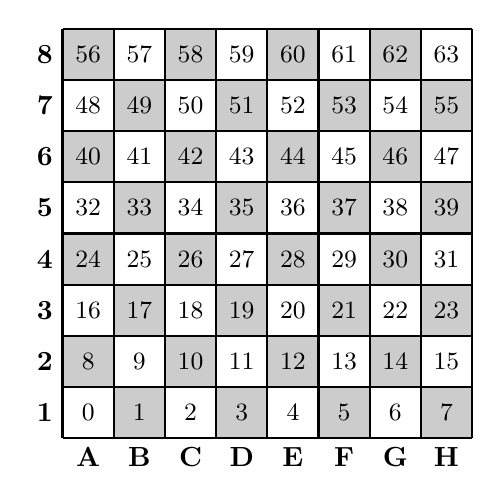
\begin{tikzpicture}[scale=0.65]
        % Draw the chessboard
        \foreach \x in {0,1,...,7} {
            \foreach \y in {0,1,...,7} {
                \pgfmathparse{mod(\x+\y,2) ? "black!20" : "white"}
                \edef\col{\pgfmathresult}
                \fill[\col] (\x,\y) rectangle (\x+1,\y+1);
                
                % Calculate the square index
                \pgfmathtruncatemacro{\num}{\x + 8*\y}
                % Add the number to the square
                \node at (\x+0.5,\y+0.5) {\small \num};
            }
        }

        % Add column labels (A-H)
        \foreach \x [count=\i from 0] in {A, B, C, D, E, F, G, H} {
            % \node[above] at (\i+0.5, 8) {\textbf{\x}}; % Top labels
            \node[below] at (\i+0.5, 0) {\textbf{\x}}; % Bottom labels
        }

        % Add row labels (1-8)
        \foreach \y [count=\i from 0] in {1, 2, 3, 4, 5, 6, 7, 8} {
            \node[left] at (0, \i+0.5) {\textbf{\y}}; % Left labels
            % \node[right] at (8, \i+0.5) {\textbf{\y}}; % Right labels
        }

        % Draw the grid
        \draw[thick] (0,0) grid (8,8);
    \end{tikzpicture}
    \caption{Little-Endian Rank-File Mapping with Coordinates.}
    \label{fig:lerf}
\end{figure}

\noindent \parbox{\textwidth}{There are bitboards for all pieces (\texttt{bitboard\_all}), for each piece color (\texttt{bitboard\_color[0]} and \texttt{bitboard\_color[1]}), and for each piece type (\texttt{bitboard\_piece[Piece]} like \texttt{bitboard\_piece[Piece::W\_QUEEN]})}.

\vspace{1em}

\noindent To identify ray directions on the board, we used the compass rose:

\begin{center}
    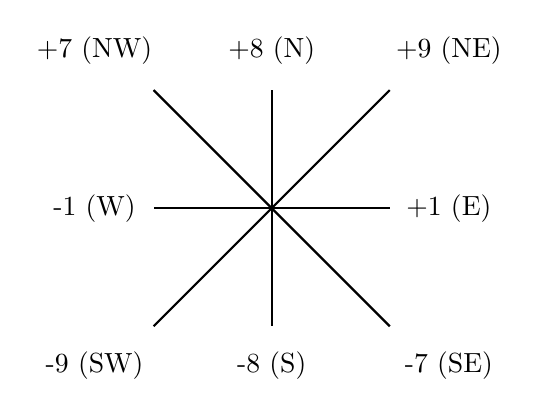
\begin{tikzpicture}
        \node at (0, 2) {+8 (N)};
        \node at (2.25, 2) {+9 (NE)};
        \node at (-2.25, 2) {+7 (NW)};
        \node at (2.25, 0) {+1 (E)};
        \node at (-2.25, 0) {-1 (W)};
        \node at (0, -2) {-8 (S)};
        \node at (2.25, -2) {-7 (SE)};
        \node at (-2.25, -2) {-9 (SW)};
        \draw[thick] (0, 0) -- (0, 1.5);
        \draw[thick] (0, 0) -- (1.5, 1.5);
        \draw[thick] (0, 0) -- (-1.5, 1.5);
        \draw[thick] (0, 0) -- (1.5, 0);
        \draw[thick] (0, 0) -- (-1.5, 0);
        \draw[thick] (0, 0) -- (0, -1.5);
        \draw[thick] (0, 0) -- (1.5, -1.5);
        \draw[thick] (0, 0) -- (-1.5, -1.5);
    \end{tikzpicture}
\end{center}

\noindent This means that, to get the numerical value that identifies the square to the north-east of a given square, you only need to add 9. For example, given the square $f6$ (45), the north-east square $g7$ has a value of 54 (45 + 9 = 54). It is really effective for sliding pieces to calculate their attacks.

\subsubsection{Transposition table}

The transposition table contains a list of entries. These entries are defined as a storage of information about a specific chess position, including its Zobrist key, evaluation score, best move, node type, and search depth.

\vspace{1em}

\noindent The use of this will be discussed in Section~\ref{sec:tt}.

\subsubsection{History}

It contains a circular array (\texttt{uint64\_t positions[HISTORY\_MAX\_SIZE]} with a position index that runs circularly \texttt{int next\_position\_index}) to store the hashes of previous board positions, ensuring efficient memory usage and quick access. This is essential for detecting threefold repetitions. Additionally, it provides functions to add new positions, remove the most recent ones, and clear the history when needed. The array is implemented with a fixed size (\texttt{HISTORY\_MAX\_SIZE}) of \(128\), defined as a power of two, to optimize indexing operations.

\vspace{1em}

\noindent The detection of threefold repetition is performed by comparing the hash of the current position with the hashes stored in the history. If the same hash appears at least twice, it indicates that the position has been repeated three times.

\subsubsection{Move generator information}

TODO

\subsubsection{Precomputed Data}

Precomputed data refers to information that is calculated and stored in advance to accelerate runtime operations. It reduces the need for repetitive calculations during gameplay. This approach allows the engine to focus on more computationally intensive tasks, such as search and evaluation.

The following types of precomputed data are used in AlphaDeepChess:

\begin{itemize}
    \item Piece-Square Tables: These tables assign a static value to each piece on every square of the board, reflecting its positional strength. For example, pawns are more valuable in the center of the board, while knights are stronger when placed near the middle. These are used for evaluation.
    
\begin{lstlisting}[breaklines=true, frame=single, caption={Initialization of knight piece-square table}]
static constexpr int KNIGHT_PIECE_SQUARE_TABLE[64] = {
    -50, -40, -30, -30, -30, -30, -40, -50,
    -40, -20, 0,   0,   0,   0,   -20, -40,
    -30, 0,   10,  15,  15,  10,  0,   -30,
    -30, 5,   15,  20,  20,  15,  5,   -30,
    -30, 0,   15,  20,  20,  15,  0,   -30,
    -30, 5,   10,  15,  15,  10,  5,   -30,
    -40, -20, 0,   5,   5,   0,   -20, -40,
    -50, -40, -30, -30, -30, -30, -40, -50
};
\end{lstlisting}
    
    \item Piece Attack Tables: Precomputed bitboards that represent the attack patterns of each piece type from every square on the board. These masks are used to quickly determine legal moves and attacked squares and they are also used in evaluation.
    
\begin{lstlisting}[breaklines=true, frame=single, caption={Initialization of bishop attack tables}]
constexpr uint64_t calculate_bishop_moves(Square square, uint64_t blockers)
{
    assert(square.is_valid());

    uint64_t moves_mask = 0ULL;

    const Direction dirs[4] = {NORTH_EAST, NORTH_WEST, SOUTH_EAST, SOUTH_WEST};

    for (const Direction dir : dirs) {

        Square aux_sq = square;
        aux_sq.to_direction(dir);

        while (aux_sq.is_valid()) {

            moves_mask |= aux_sq.mask();

            if (blockers & aux_sq.mask()) {
                break;   // if there is a blocker in the square we stop in this direction
            }
            else {
                aux_sq.to_direction(dir);
            }
        }
    }

    return moves_mask;
}
\end{lstlisting}

    \item Ray Directions: Precomputed arrays that store the sliding attack directions for each square. These are used to efficiently calculate moves for sliding pieces during move generation.
    
\begin{lstlisting}[breaklines=true, frame=single, caption={Initialization of directions masks}]
static constexpr const std::array<std::array<uint64_t, 64>, 64> init_direction_mask()
{
    std::array<std::array<uint64_t, 64>, 64> PRECOMPUTED_DIR_MASK = {};

    for (Square sq1 = Square::A1; sq1.is_valid(); sq1++) {
        for (Square sq2 = Square::A1; sq2.is_valid(); sq2++) {

            if (sq1.row() == sq2.row()) {
                PRECOMPUTED_DIR_MASK[sq1][sq2] = get_row_mask(sq1.row());
            }
            else if (sq1.col() == sq2.col()) {
                PRECOMPUTED_DIR_MASK[sq1][sq2] = get_col_mask(sq1.col());
            }
            else if (squares_in_same_diagonal(sq1, sq2)) {
                PRECOMPUTED_DIR_MASK[sq1][sq2] = get_diagonal_mask(sq1.diagonal());
            }
            else if (squares_in_same_antidiagonal(sq1, sq2)) {
                PRECOMPUTED_DIR_MASK[sq1][sq2] = get_antidiagonal_mask(sq1.antidiagonal());
            }
            else {
                PRECOMPUTED_DIR_MASK[sq1][sq2] = 0ULL;
            }
        }
    }

    return PRECOMPUTED_DIR_MASK;
}
\end{lstlisting}
    
    \item Zobrist Hash Seeds: Randomly generated 64-bit numbers used for Zobrist hashing. Each piece-square combination, castling right, en passant square, and side to move is assigned a unique random value.
    
\begin{lstlisting}[breaklines=true, frame=single, caption={Initialization of seeds}]
static void init_random_numbers_only_once()
{
    static bool initialized = false;

    if (initialized) {
        return;
    }

#ifndef NDEBUG
    const uint64_t SEED = 123456789ULL;
    std::mt19937_64 gen(SEED);   // Use constant seed in debug mode
#else
    std::random_device rd;
    std::mt19937_64 gen(rd());   // Use random seed in release mode
#endif

    std::uniform_int_distribution<uint64_t> dis;

    for (Square sq = Square::A1; sq.is_valid(); sq++) {
        for (int p = 0; p < 12; p++) {
            square_piece_seed[sq.value()][p] = dis(gen);
        }
    }

    for (auto& elem : en_passant_seed) {
        elem = dis(gen);
    }

    king_white_castle_seed = dis(gen);
    queen_white_castle_seed = dis(gen);
    king_black_castle_seed = dis(gen);
    queen_black_castle_seed = dis(gen);

    black_to_move_seed = dis(gen);

    initialized = true;
}
\end{lstlisting}

\end{itemize}

\subsection{Evaluation}

In addition to the basic information that is mentioned in Section~\ref{sec:evaluation}, in order to calculate the game phase, we can perform a dynamic evaluation (tampering evaluation): evaluate twice, once as if we were in the middlegame and once as if we were in the endgame. The final evaluation will be the sum of both, but each with a different weight. To do this, we calculate the middlegame percentage (24 pieces means 100\% middlegame) and the endgame percentage (0 pieces = 100\% endgame).

\begin{align*}
\text{Evaluation} &= middlegame\% \cdot eval\_middlegame + endgame\% \cdot eval\_endgame
\end{align*}

\vspace{1em}

\begin{lstlisting}[breaklines=true, frame=single, caption={Counting pieces and depending on game phase evaluation.}]
int evaluate_position(Board& board)
{
    board.update_attacks_bb();

    int middlegame_eval = 0;
    int endgame_eval = 0;

    const int middlegame_percentage = calculate_middlegame_percentage(board);
    const int endgame_percentage = 24 - calculate_middlegame_percentage(board);

    uint64_t pieces = board.get_bitboard_all();

    while (pieces) {

        const Square square(pop_lsb(pieces));
        const Piece piece = board.get_piece(square);
        const ChessColor color = get_color(piece);
        const int piece_raw_value = raw_value(piece);
        const int bonus_middlegame = PrecomputedEvalData::get_piece_square_table<PST_TYPE_MIDDLEGAME>(piece, square);
        const int bonus_endgame = PrecomputedEvalData::get_piece_square_table<PST_TYPE_ENDGAME>(piece, square);

        const int piece_value_middlegame = piece_raw_value + bonus_middlegame;
        const int piece_value_endgame = piece_raw_value + bonus_endgame;

        middlegame_eval += is_white(color) ? piece_value_middlegame : -piece_value_middlegame;
        endgame_eval += is_white(color) ? piece_value_endgame : -piece_value_endgame;
    }
    const int blended_eval = (middlegame_eval * middlegame_percentage + endgame_eval * endgame_percentage) / 24;

    return blended_eval;
}
\end{lstlisting}

\begin{lstlisting}[breaklines=true, frame=single, caption={King safety, piece mobility, depending on game phase evaluation.}]
int evaluate_position(Board& board)
{
    board.update_attacks_bb();

    int middlegame_eval = 0;
    int endgame_eval = 0;

    const int middlegame_percentage = calculate_middlegame_percentage(board);
    const int endgame_percentage = 24 - calculate_middlegame_percentage(board);

    const Square white_king_sq = lsb(board.get_bitboard_piece(Piece::W_KING));
    const Square black_king_sq = lsb(board.get_bitboard_piece(Piece::B_KING));

    uint64_t pieces = board.get_bitboard_all();

    while (pieces) {

        const Square square(pop_lsb(pieces));
        const Piece piece = board.get_piece(square);
        const ChessColor color = get_color(piece);
        const int piece_raw_value = raw_value(piece);
        const int bonus_middlegame = PrecomputedEvalData::get_piece_square_table<PST_TYPE_MIDDLEGAME>(piece, square);
        const int bonus_endgame = PrecomputedEvalData::get_piece_square_table<PST_TYPE_ENDGAME>(piece, square);
        const int mobility = mobility_piece_score(square, piece, board);

        const int piece_value_middlegame = piece_raw_value + bonus_middlegame + mobility;
        const int piece_value_endgame = piece_raw_value + bonus_endgame + mobility;

        middlegame_eval += is_white(color) ? piece_value_middlegame : -piece_value_middlegame;
        endgame_eval += is_white(color) ? piece_value_endgame : -piece_value_endgame;
    }

    const int king_safety_penality_white = king_safety_penalization<ChessColor::WHITE>(white_king_sq, board);
    const int king_safety_penality_black = king_safety_penalization<ChessColor::BLACK>(black_king_sq, board);
    const int king_safety_penality = king_safety_penality_black - king_safety_penality_white;

    const int king_shield_bonus_white = king_shield<ChessColor::WHITE>(white_king_sq, board);
    const int king_shield_bonus_black = king_shield<ChessColor::BLACK>(black_king_sq, board);
    const int king_shield_bonus = king_shield_bonus_white - king_shield_bonus_black;

    middlegame_eval += king_shield_bonus + king_safety_penality;

    const int blended_eval = (middlegame_eval * middlegame_percentage + endgame_eval * endgame_percentage) / 24;

    return blended_eval;
}
\end{lstlisting}

\begin{lstlisting}[breaklines=true, frame=single, caption={Different pawn square values depending on game phase.}]
// Opening and Middlegame pawn square values
static constexpr int PAWN_PIECE_SQUARE_TABLE[64] = {
    0,   0,   0,   0,   0,   0,   0,   0,
    50,  50,  50,  50,  50,  50,  50,  50,
    10,  10,  20,  30,  30,  20,  10,  10,
    5,   5,   10,  25,  25,  10,  5,   5,
    0,   0,  0,   20,  20,  0,   -5,  0,
    5,   -5,  -10, 0,   0,   -10, -5,  5,
    5,   10,  10,  -20, -20, 10,  10,  5,
    0,   0,   0,   0,   0,   0,   0,   0
};

// Endgame pawn square values
static constexpr int PAWN_ENDGAME_SQUARE_TABLE[64] = {
    0,   0,   0,   0,   0,   0,   0,   0,
    80,  80,  80,  80,  80,  80,  80,  80,
    50,  50,  50,  50,  50,  50,  50,  50,
    30,  30,  30,  30,  30,  30,  30,  30,
    20,  20,  20,  20,  20,  20,  20,  20,
    10,  10,  10,  10,  10,  10,  10,  10,
    10,  10,  10,  10,  10,  10,  10,  10,
    0,   0,   0,   0,   0,   0,   0,   0
};
\end{lstlisting}

\subsection{Move generator}

Calculating the legal moves in a chess position is a more difficult and tedious task than it might seem, mainly due to the unintuitive rules of en passant and castling, and it is also difficult to restrict the moves of pinned pieces.~\cite{GenerateLegalMovesEfficiently}

\vspace{1em}

\noindent To create an efficient move generator, we will be using bitboards. The steps to generate legal movements efficiently are the following:

\begin{itemize}
  \item Calculate the bitboard of attacked squares by the waiting side.
  \item Calculate bitboard of pinned pieces.
  \item Generate the legal moves of each piece of the side whose turn is, knowing that the king cannot move to any attacked square and that pinned pieces can only move in the direction of the pin.
  \item Generate the special legal moves like en passant and castling.
\end{itemize}

TODO: insert some of the code of move generator

\subsection{Move ordering}

Order the legal moves from most to least likely to be the best move in the position. The sooner we explore the best move, the more branches of the tree will be pruned. To do this, we use the MVV-LVA heuristic (most valuable victim, least valuable aggressor). We give higher scores to capturing a low-value piece over a higher-value piece. Capturing a queen with a pawn scores highly. We also give a bonus to piece promotions.

\vspace{1em}

TO DO: insert code of move ordering

\subsubsection{Killer moves}

A killer move is a non-capturing (quiet) move that previously caused a beta-cutoff during the search in a sibling node or any other branch at the same depth in the game tree. These moves are often strong candidates, as they have previously led to pruning in similar positions. Promoting them early in the move ordering increases the chances of early cutoffs, which improves search efficiency.

\vspace{1em}

\noindent To take advantage of this heuristic we store up to two killer moves for each search depth. During move ordering, these killer moves are given a bonus score, allowing them to be explored before other quiet moves.

\vspace{1em}

TODO: insert code of killer moves

\subsection{The Core: Search Algorithm}

The core of the chess engine is its search algorithm, in this case alpha-beta pruning algorithm. The entire game tree is generated up to a selected maximum depth. At each node, the next player evaluates the position and during execution, the values of alpha and beta are updated. Pruning is performed when a branch of the tree is detected as irrelevant because the evaluation being examined is worse than the current value of alpha or beta for MAX or MIN, respectively.

\vspace{1em}

\noindent Therefore, the following events happen at each node of the tree:

\begin{itemize}
    \item Check if we are at an end node because of a checkmate, a draw by triple repetition, the 50-move rule, or because we have reached the maximum selected depth.
    \item Evaluate the position: a positive value (+) means that White has an advantage, and a negative value (-) means that Black has an advantage. A limit is set that represents mate in one; we have arbitrarily chosen 3,200,000.
    \item Generate legal moves: create a list of every possible legal move in the position.
    \item Order the legal moves: from greatest to least intuition of being the best move for the position. The sooner we explore the best move, the more branches of the tree will be pruned.
    \item Explore each of the legal moves from the position in order, update the evaluation, the value of alpha and beta, and check if we can perform pruning.
\end{itemize}

\vspace{1em}

\begin{lstlisting}[breaklines=true, frame=single, caption={Alpha-Beta search.}]
template<SearchType searchType>
static int alpha_beta_search(std::atomic<bool>& stop, int depth, int ply, int alpha, int beta, SearchContext& context)
{
    // ...

    MoveList moves;
    bool isCheck;
    generate_legal_moves<ALL_MOVES>(moves, board, &isCheck);
    // Verify ending position: checkmate, stalemate, fifty-move rule counter...

    int final_node_evaluation = MAXIMIZING_WHITE ? -INF_EVAL : +INF_EVAL;
    const GameState game_state = board.state();

    order_moves(moves, board, ply);

    for (int i = 0; i < moves.size(); i++) {
        // ...
        constexpr SearchType nextSearchType = MAXIMIZING_WHITE ? MINIMIZE_BLACK : MAXIMIZE_WHITE;

        board.make_move(moves[i]);
        int eval = alpha_beta_search<nextSearchType>(stop, depth - 1, ply + 1, alpha, beta, context);
        board.unmake_move(moves[i], game_state);
        History::pop_position();

        if constexpr (MAXIMIZING_WHITE) {
            // ...

            final_node_evaluation = std::max(final_node_evaluation, eval);
            alpha = std::max(alpha, eval);

            if (final_node_evaluation >= beta) {
                // ...
                break;   // beta cutoff
            }
        }
        else if (MINIMIZING_BLACK) {
            // ...

            final_node_evaluation = std::min(final_node_evaluation, eval);
            beta = std::min(beta, eval);

            if (final_node_evaluation <= alpha) {
                // ...
                break;   // alpha cutoff
            }
        }
    }

    return final_node_evaluation;
}
\end{lstlisting}

\subsubsection{Search: iterative deepening}

At what depth do we decide to search? Actually, the simplest thing is to perform an infinite search, first searching at depth 1, then 2, then 3\ldots to infinity. The engine will update the evaluation and the best move for the position in each iteration. Simply by signaling \textit{stop} the search will stop.

\vspace{1em}

\begin{lstlisting}[breaklines=true, frame=single, caption={Iterative deepening.}]
static void iterative_deepening(std::atomic<bool>& stop, SearchResults& results, int max_depth, SearchContext& context)
{
    // ...

    int alpha = -INF_EVAL;
    int beta = +INF_EVAL;

    for (int depth = 1; depth <= max_depth; depth++) {
        context.bestMoveInIteration = Move::null();
        context.bestEvalInIteration = is_white(side_to_move) ? -INF_EVAL : +INF_EVAL;

        // ...

        is_white(side_to_move) ? alpha_beta_search<MAXIMIZE_WHITE>(stop, depth, 0, alpha, beta, context)
                               : alpha_beta_search<MINIMIZE_BLACK>(stop, depth, 0, alpha, beta, context);

        // ...

        context.bestMoveFound = context.bestMoveInIteration;
        context.bestEvalFound = context.bestEvalInIteration;

        assert(context.bestMoveFound.is_valid());

        insert_new_result(results, depth, context.bestEvalFound, context.bestMoveFound);

        if (abs(context.bestEvalFound) > MATE_THRESHOLD) {
            break;   // We found a checkmate, we stop because we cant find a shorter checkMate
        }
    }
}
\end{lstlisting}

\subsubsection{Search: aspiration window}

Aspiration window's main objetive is to reduce the number of nodes to explore by simply restricting the range of alpha and beta values (window). A search is performed with this narrow window. If the position evaluation falls within the window, it is accepted as valid and additional node exploration is avoided. However, if the evaluation is outside the limits of the window (when a fail-low or fail-high occurs), the window is expanded to the extreme values (-INF and +INF) and a new search is performed to obtain an accurate evaluation:

\begin{lstlisting}[breaklines=true, frame=single, caption={Aspiration window.}]
static void iterative_deepening(std::atomic<bool>& stop, SearchResults& results, int max_depth, SearchContext& context)
{
    // ...

    int alpha = -INF_EVAL;
    int beta = +INF_EVAL;

    for (int depth = 1; depth <= max_depth; depth++) {
        context.bestMoveInIteration = Move::null();
        context.bestEvalInIteration = is_white(side_to_move) ? -INF_EVAL : +INF_EVAL;

        // if it is not the first iteration, adjust alpha and beta
        if (depth > 1) {
            alpha = context.bestEvalFound - ASPIRATION_MARGIN;
            beta  = context.bestEvalFound + ASPIRATION_MARGIN;
        }

        is_white(side_to_move) ? alpha_beta_search<MAXIMIZE_WHITE>(stop, depth, 0, alpha, beta, context)
                               : alpha_beta_search<MINIMIZE_BLACK>(stop, depth, 0, alpha, beta, context);

        // if the evaluation is out of bounds of the window, redo the search with -INF_EVAL and +INF_EVAL
        if (context.bestEvalInIteration <= alpha || context.bestEvalInIteration >= beta) {
            alpha = -INF_EVAL;
            beta  = +INF_EVAL;

            is_white(side_to_move) ? alpha_beta_search<MAXIMIZE_WHITE>(stop, depth, 0, alpha, beta, context)
                                   : alpha_beta_search<MINIMIZE_BLACK>(stop, depth, 0, alpha, beta, context);
        }

        // ...
    }
}
\end{lstlisting}

\subsubsection{Search: horizon effect, quiescence search}

What happens if, upon reaching maximum depth, we evaluate the position in the middle of a piece exchange? For example, if a queen captures a pawn. It will seem like we have won a pawn, but on the next move, another pawn captures the queen, and now we lose a queen. This is known as the horizon effect. To avoid this, when we reach the end of the tree at maximum depth, we must extend the search to include only piece captures. This is known as quiescence search.

\vspace{1em}

\noindent The purpose of this search is only to stop the search and evaluate quiet positions, where there is no capture or tactical movement.

\vspace{1em}

\begin{lstlisting}[breaklines=true, frame=single, caption={Quiescence search implementation.}]
template<SearchType searchType>
static int quiescence_search(bool& stop, int ply, int alpha, int beta, SearchContext& context)
{
    constexpr bool MAXIMIZING_WHITE = searchType == MAXIMIZE_WHITE;
    constexpr bool MINIMIZING_BLACK = searchType == MINIMIZE_BLACK;

    Board& board = context.board;
    const uint64_t zobrist_key = board.state().get_zobrist_key();

    const uint8_t fifty_move_rule_counter = board.state().fifty_move_rule_counter();
    const bool fify_move_rule_draw = fifty_move_rule_counter >= 100U;

    if (History::threefold_repetition_detected(fifty_move_rule_counter) || fify_move_rule_draw) {
        return 0;
    }

    int static_evaluation = evaluate_position(board);

    if (ply >= MAX_PLY) {
        return static_evaluation;
    }

    if constexpr (MAXIMIZING_WHITE) {
        if (static_evaluation >= beta) {
            return beta;   // beta cutoff
        }
        alpha = std::max(alpha, static_evaluation);
    }
    else if constexpr (MINIMIZING_BLACK) {
        if (static_evaluation <= alpha) {
            return alpha;   // Alpha cutoff
        }
        beta = std::min(beta, static_evaluation);
    }

    MoveList capture_moves;
    generate_legal_moves<ONLY_CAPTURES>(capture_moves, board);

    if (capture_moves.size() == 0) {
        return static_evaluation;   // No captures: return static evaluation
    }

    order_moves(capture_moves, board, ply);

    const GameState game_state = board.state();
    int final_node_evaluation = static_evaluation;

    for (int i = 0; i < capture_moves.size(); i++) {

        if (stop) {
            return 0;
        }

        constexpr SearchType nextSearchType = MAXIMIZING_WHITE ? MINIMIZE_BLACK : MAXIMIZE_WHITE;

        History::push_position(zobrist_key);
        board.make_move(capture_moves[i]);
        int eval = quiescence_search<nextSearchType>(stop, ply + 1, alpha, beta, context);
        board.unmake_move(capture_moves[i], game_state);
        History::pop_position();

        if constexpr (MAXIMIZING_WHITE) {
            final_node_evaluation = std::max(final_node_evaluation, eval);
            alpha = std::max(alpha, eval);

            if (final_node_evaluation >= beta) {
                break;   // Beta cutoff
            }
        }
        else if constexpr (MINIMIZING_BLACK) {
            final_node_evaluation = std::min(final_node_evaluation, eval);
            beta = std::min(beta, eval);

            if (final_node_evaluation <= alpha) {
                break;   // Alpha cutoff
            }
        }
    }

    return final_node_evaluation;
}
\end{lstlisting}

\subsection{UCI}

Universal Chess Interface specifications are independent of the operating system. To ensure the synchronization of the engine with the GUI, a \texttt{isready} command is sent and engine should respond with \texttt{readyok}.

\vspace{1em}

\noindent The engine must be capable of continuously processing input from standard input, even during evaluation. Moreover, if an unknown command is received, it should be ignored.

\vspace{1em}

\noindent The move format is in long algebraic notation which means sending two squares coordinates like \texttt{e2e4} or \texttt{b1c3} independently of the type of piece because the engine must be the one checking that the movement is legal.

\vspace{1em}

\noindent Some of the most important commands are the following:

\begin{itemize}
    \item \parbox{\textwidth}{\texttt{position [fen <fenstring> | startpos | actualpos] moves <move1> \ldots <movei>}}: sets the current position of the board to the FEN string or make the list of moves from starting position or current position.
    \item \texttt{go}: starts evaluating the current position. Some important subparameters are:
    \begin{itemize}
        \item \texttt{depth <x>}: specifies the number of \texttt{x} plies to search.
        \item \texttt{movetime <x>}: specifies the number of \texttt{x} seconds to search. 
    \end{itemize}
    \item \texttt{stop}: stops evaluation if it is running.
\end{itemize}

\section{Improvements}

Some improvements and new structures were later added for different versions: transposition tables, Zobrist hashing, table entries, PEXT instructions, search multithread and search reductions that will be discussed and analysed below.

\subsection{Transposition Table}
\label{sec:tt}

\noindent The basic implementation of the chess engine generates a large amount of redundant calculations due to transpositions: situations in which the same board position is reached through different sequences of moves in the game tree.
\noindent Figure~\ref{fig:transposition_example} illustrates a position that can arise through multiple move orders. Where the white king could go to the g3 square from multiple paths.

\begin{figure}[H]
    \centering
    \begin{minipage}{0.6\textwidth}
        \centering
        \newchessgame
        \chessboard[
            showmover=false,
            setfen=8/2k5/3p4/p2P1p2/P2P1P2/8/8/2K5 w - - 0 1,
            pgfstyle=straightmove, color=blue,
            markmoves={c1-e3,e3-g3,c1-g1,g1-g3},
            arrow=to
        ]
    \end{minipage}
    \caption{Lasker-Reichhelm Position, transposition example}
    \label{fig:transposition_example}
\end{figure}

\vspace{1em}

\noindent Taking advantage of the concept of dynamic programming, we are going to create a look-up table of chess positions and its evaluation. So if we encounter the same position again, the evaluation is already precalculated. However, we ask ourselves the following question: how much space does the look-up table take up if there are an astronomical amount of chess positions? What we can do is assign a hash to each position and make the table index the last bits of the hash. The larger the table, the less likely access collisions will be. We also want a hash that is fast to calculate and has collision-reducing properties; for this, we will use the Zobrist hashing technique in the following subsection.

\vspace{1em}

\subsubsection{Zobrist Hashing}

Zobrist Hashing is a technique to transform a board position of arbitrary size into a number of a set length, with an equal distribution over all possible numbers invented by Albert Zobrist. (\cite{ZobristHashing})

\vspace{1em}

\noindent To generate a 64-bit hash for a position, the following steps are followed:

\begin{itemize}
  \item There are 12 different types of chess pieces. For each of the 64 squares on the board, we generate 12 random 64-bit integers. That is, each piece-square combination is assigned a unique random value. This initialization step is performed only once when the program starts.
  \item The hash value for a given position is computed by performing the XOR operation between the hash accumulator and the random value corresponding to each piece on its square.
  \item In addition to the pieces, we also include:
  \begin{itemize}
    \item A random value for the side to move.
    \item One random value to account for the possibility of an en passant capture.
    \item One random value per possible castling move.
  \end{itemize}
  \item These random values are useful so that even slightly different positions produce very different hash values. This greatly reduces the chance of collisions.
  \item The XOR operation is used not only because it is computationally inexpensive, but also because it is reversible. This means that when a move is made or undone, we can update the hash incrementally by applying XOR only to the affected squares, without needing to recompute the entire hash.
\end{itemize}

\begin{lstlisting}[breaklines=true, frame=single, caption={Code example to calculate zobrist hash of position}, label={lst:zobrist_calculate_hash}]
/**
 * @brief Calculate zobrist hash of position
 * 
 * @param[in] position board containing the chess position
 * 
 * @return the hash key of the chess position
 * 
 */
static uint64_t hash(const Board& position)
{
    // initialize the random numbers only once
    init_random_numbers_only_once();   

    uint64_t hash = 0ULL;

    for (Square square = Square::A1; square.is_valid(); square++) {
        const Piece piece = position.get_piece(square);
        if (piece != Piece::EMPTY) {
            hash ^= get_seed(square, piece);
        }
    }
    const GameState state = position.state();

    const Square eps_square = state.en_passant_square();
    if (eps_square.is_valid()) {
        hash ^= get_en_passant_seed(eps_square.col());
    }

    if (state.castle_king_white()) {
        hash ^= get_king_white_castle_seed();
    }
    if (state.castle_queen_white()) {
        hash ^= get_queen_white_castle_seed();
    }
    if (state.castle_king_black()) {
        hash ^= get_king_black_castle_seed();
    }
    if (state.castle_queen_black()) {
        hash ^= get_queen_black_castle_seed();
    }

    if (state.side_to_move() == ChessColor::BLACK) {
        hash ^= get_black_to_move_seed();
    }

    return hash;
}
\end{lstlisting}

\subsubsection{Table Entry}

Each entry in the transposition table stores the following information:

\begin{itemize}
  \item Zobrist Hash: The full 64-bit hash of the position. This is used to verify that the entry corresponds to the current position and to detect possible index collisions in the table.
  \item Evaluation: The numerical evaluation of the position, as computed by the evaluation function.
  \item Depth: The depth at which the evaluation was calculated. A deeper search could potentially yield a more accurate evaluation, so this value helps determine whether a new evaluation should overwrite the existing one.
  \item Node Type: Indicates the type of node stored:
  \begin{itemize}
    \item \texttt{EXACT} the evaluation is precise for this position.
    \item \texttt{UPPERBOUND} the evaluation is an upper bound, typically resulting from an alpha cutoff.
    \item \texttt{LOWERBOUND} the evaluation is a lower bound, typically resulting from a beta cutoff.
    \item \texttt{FAILED} entry is empty or with invalid information.
  \end{itemize}
\end{itemize}

\begin{lstlisting}[breaklines=true, frame=single, caption={Code example transposition table entry}, label={lst:transposition_table_entry}]
class TranspositionTable::Entry
{
    uint64_t key; // full Zobrist key of the chess position

    int evaluation; // Score of the chess position

    Move move; // Best move found for the position.

    NodeType type; // FAILED, EXACT, LOWERBOUND, UPPERBOUND

    int8_t depth; // At which the position was evaluated
...
}
\end{lstlisting}

\subsubsection{Collisions}

As discussed earlier, index collisions in the transposition table are handled by verifying the full Zobrist hash stored in the entry. However, it is still theoretically possible for a full hash collision to occur, that is two different positions producing the same hash.

\vspace{1em}

\noindent This scenario is extremely rare. With 64-bit hashes, there are $2^{64}$ possible unique values, which is more than sufficient for practical purposes. In the unlikely event of a true hash collision, it could result in an incorrect evaluation being reused for a different position.

\subsubsection{Analysis}

To evaluate the improvement introduced by the transposition table, we conducted a 100-game tournament against the basic version of the engine. We selected 50 random starting positions from an opening book and played each position twice, alternating colors to ensure fairness. Each bot has 4 seconds to think per move.

\begin{center}
\begin{figure}[H]
    \centering
    \ResultBar{15cm}{0.5cm}{46}{22}{32}
    \caption{64MB Transposition Table bot vs basic bot}
    \label{fig:results_transposition_table_bot}
\end{figure}
\medskip
\end{center}

\noindent We see a substantial improvement by adding the transposition table with 46 wins versus 32 losses.

\subsection{Move generator with Magic Bitboards and PEXT instructions}

To identify potential performance bottlenecks, we performed profiling on the engine.

\begin{center}
    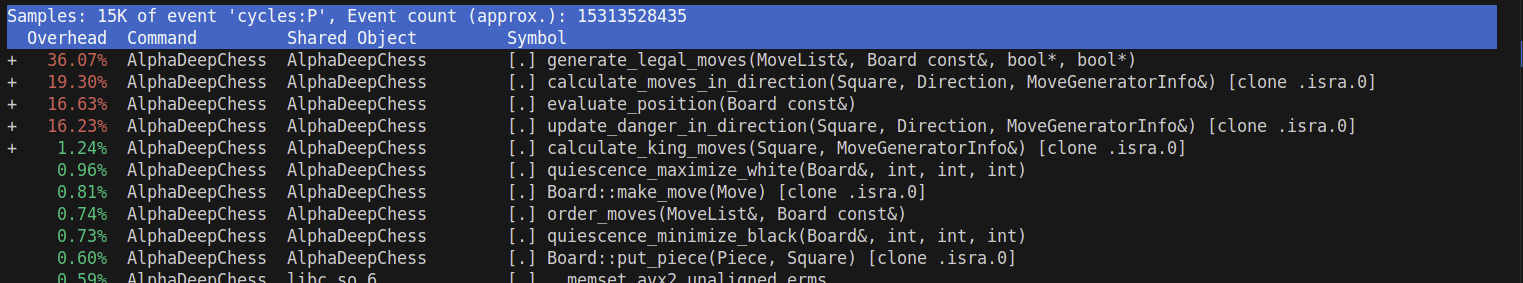
\includegraphics[width=1.0\textwidth]{Imagenes/basic_move_generator_profiling.png}
\end{center}

\noindent Profiling results show that most part of the total execution time is spent in the generate legal moves function. Therefore, optimizing this component is expected to lead to significant performance improvements.

\subsubsection{Magic bitboards}

We can create a look up table of all the rook and bishop moves for each square on the board and for each combination of pieces that blocks the path of the slider piece (blockers  bitboard). Basically we need a hash table to store rook and bishop moves indexed by square and bitboard of blockers. The problem is that this table could be very big.~\cite{MagicBitboards}

\vspace{1em}

\noindent Magic bitboards technique used to reduce the size of the look up table. We cut off unnecesary information in the blockers bitboard, excluding the board borders and the squares outside its attack pattern.

\vspace{1em}

A \textbf{magic number} is a multiplier to the bitboard of blockers with the following properties:

\begin{itemize}
  \item Preserves relevant blocker information: 
  The nearest blockers along a piece's movement direction are preserved. 
  \textit{Example:} Consider a rook with two pawns in its path:
  \begin{lstlisting}[breaklines=true]
    Rook -> -> -> [Pawn1][Pawn2]
  \end{lstlisting}
  In this case, only `Pawn1` blocks the rook's movement, while `Pawn2` is irrelevant.
  \item Compresses the blocker bitboard, pushing the important bits near the most significant bit.
  \item The final multiplication must produce a unique index for each possible blocker configuration. The way to ensure the uniqueness is by brute force testing.
\end{itemize}

\noindent As illustrated in Figure~\ref{fig:magics_position}, we aim to compute the legal moves of the white rook in the given position. In practice, the only pieces that truly block the rook's path are those marked with a red circle.

\begin{figure}[H]
    \centering
    \begin{minipage}{0.6\textwidth}
        \centering
        \newchessgame
        \chessboard[
            showmover=false,
            setfen=n1bk3r/3p4/1p1p2p1/8/3R1p2/8/3p4/7n w - - 0 1,
            markstyle=circle,
            color=red, markfields={d6,f4,d2},
            color=green, markfields={c4,b4,a4,e4,d5,d3}
        ]
    \end{minipage}
    \caption{Initial chess position with white rook and blockers}
    \label{fig:magics_position}
\end{figure}

\noindent First, we mask out all pieces outside the rook's attack pattern or on the board borders, as shown in Figure~\ref{fig:magic_preprocessing}.

\begin{figure}[H]
    \centering
    \begin{minipage}[c]{0.4\textwidth}
        \centering
        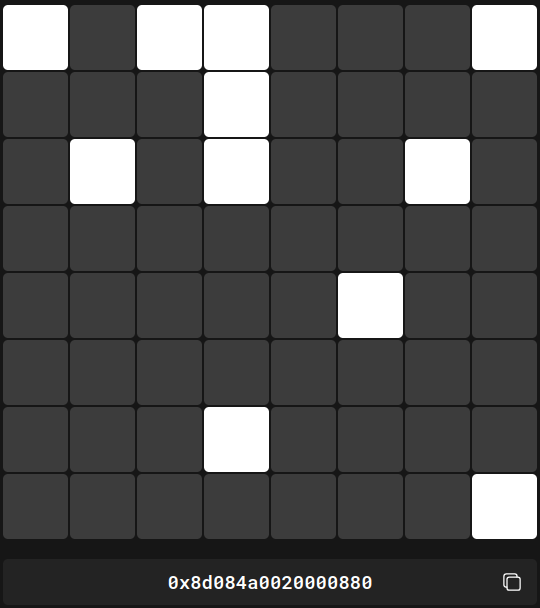
\includegraphics[width=\textwidth]{Imagenes/magics_blockers.png}
        \caption*{Original blockers bitboard}
    \end{minipage}
    \hfill
    \begin{minipage}[c]{0.1\textwidth}
        \centering
        \small$\to$
    \end{minipage}
    \hfill
    \begin{minipage}[c]{0.4\textwidth}
        \centering
        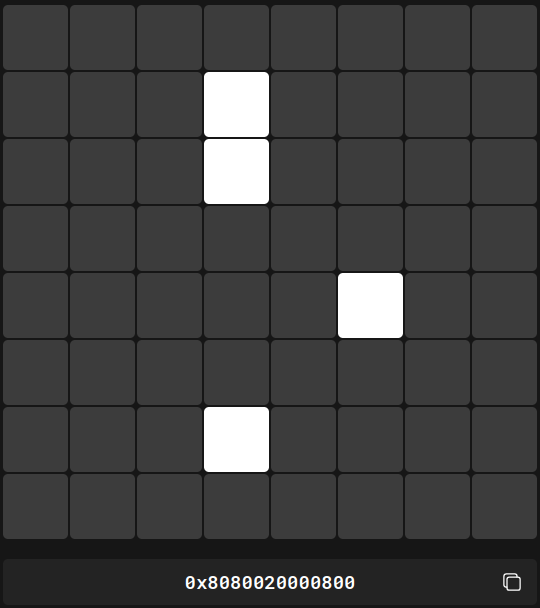
\includegraphics[width=\textwidth]{Imagenes/magics_processed_blockers.png}
        \caption*{Masked blockers bitboard}
    \end{minipage}
    \caption{Pre-processing of the blockers bitboard}
    \label{fig:magic_preprocessing}
\end{figure}

\noindent As illustrated in Figure~\ref{fig:magic_multiplication}, the masked blockers bitboard is then multiplied by the magic number. The result retains only the three relevant pawns that obstruct the rook's movement, pushing them toward the most significant bits.

\begin{figure}[H]
    \centering
    \begin{minipage}[c]{0.4\textwidth}
        \centering
        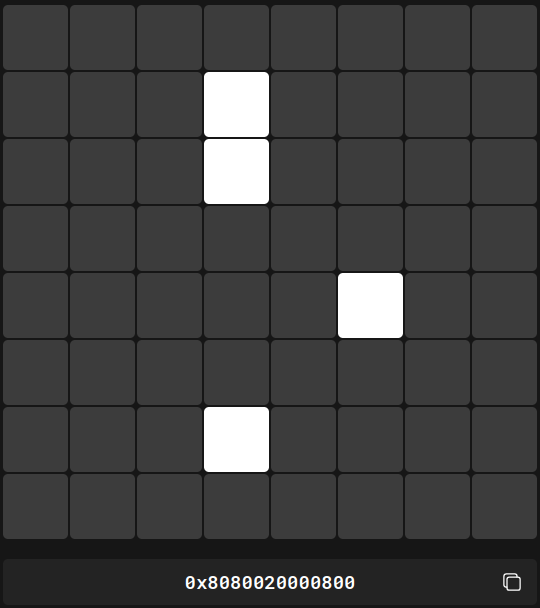
\includegraphics[width=\textwidth]{Imagenes/magics_processed_blockers.png}
        \caption*{Masked blockers bitboard}
    \end{minipage}
    \hfill
    \begin{minipage}[c]{0.1\textwidth}
        \centering
        \Huge$\times$ \\[0.5em]
        \small Magic number \\[0.5em]
        \Huge$=$
    \end{minipage}
    \hfill
    \begin{minipage}[c]{0.4\textwidth}
        \centering
        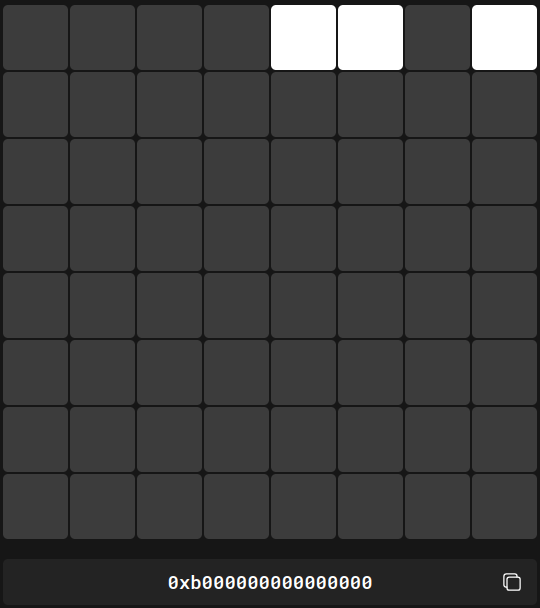
\includegraphics[width=\textwidth]{Imagenes/magics_multiplied_blockers.png}
        \caption*{Multiplied blockers bitboard}
    \end{minipage}
    \caption{Multiplication by magic number to produce an index}
    \label{fig:magic_multiplication}
\end{figure}

\noindent Next, we compress the index toward the least significant bits by shifting right by \(\,64-\)\texttt{relevant\_squares}. The number of relevant squares varies per board square; Listing~\ref{lst:rook_relevant_squares} shows this for the rook:

\begin{lstlisting}[breaklines=true, frame=single, caption={Number of relevant squares for each rook square}, label={lst:rook_relevant_squares}]
/**
 * @brief ROOK_RELEVANT_SQUARES
 * 
 * Number of squares where the rook could move
 * from each square minus the board border squares.
 */
static constexpr int ROOK_RELEVANT_SQUARES[NUM_SQUARES] =
{
    12, 11, 11, 11, 11, 11, 11, 12,
    11, 10, 10, 10, 10, 10, 10, 11,
    11, 10, 10, 10, 10, 10, 10, 11,
    11, 10, 10, 10, 10, 10, 10, 11,
    11, 10, 10, 10, 10, 10, 10, 11,
    11, 10, 10, 10, 10, 10, 10, 11,
    11, 10, 10, 10, 10, 10, 10, 11,
    12, 11, 11, 11, 11, 11, 11, 12
};
\end{lstlisting}

\vspace{1em}

\noindent The final index is thus computed as:

\begin{align*}
    \text{index}
    &= (\texttt{bitboard\_of\_blockers} \times \texttt{magic\_number})
       \;\gg\;(64 - \texttt{relevant\_squares})\,.
\end{align*}

\subsubsection{PEXT instruction}

\noindent The \texttt{PEXT} (Parallel Bits Extract) instruction—available on modern x86\_64 CPUs—extracts bits from a source operand according to a mask and packs them into the lower bits of the destination operand.~\cite{PextInstruction} It is ideally suited for computing our table index.

Figure~\ref{fig:pext_instruction_example} illustrates how \texttt{PEXT} works: it selects specific bits from register \texttt{r2}, as specified by the mask in \texttt{r3}, and packs the result into the lower bits of the destination register \texttt{r1}.

\begin{figure}[H]
    \centering
    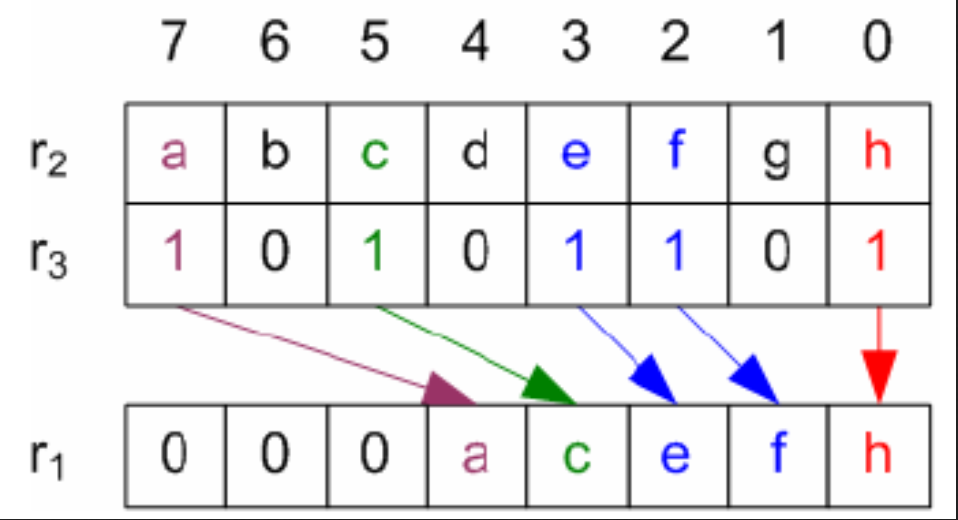
\includegraphics[width=0.5\textwidth]{Imagenes/pext.png}
    \caption{Example of the \texttt{PEXT} instruction: extracting bits from \texttt{r2} using \texttt{r3} as a mask, and storing the result in \texttt{r1}. ~\cite{PextInstruction}}
    \label{fig:pext_instruction_example}
\end{figure}

\noindent For our previous example (see Figure~\ref{fig:magics_position}), we only need the full bitboard of blockers and the rook’s attack pattern (excluding the borders to reduce space), as illustrated in Figure~\ref{fig:pext_bitboards}.

\begin{figure}[H]
    \centering
    \begin{minipage}[c]{0.3\textwidth}
        \centering
        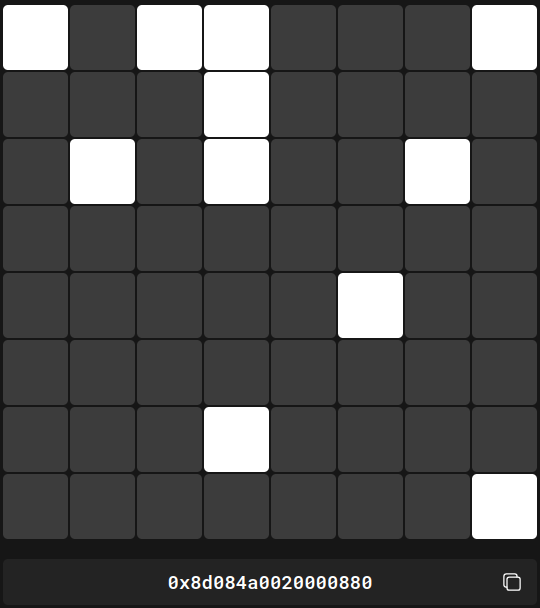
\includegraphics[width=\textwidth]{Imagenes/magics_blockers.png}
        \caption*{Blockers bitboard}
    \end{minipage}
    \hfill
    \begin{minipage}[c]{0.3\textwidth}
        \centering
        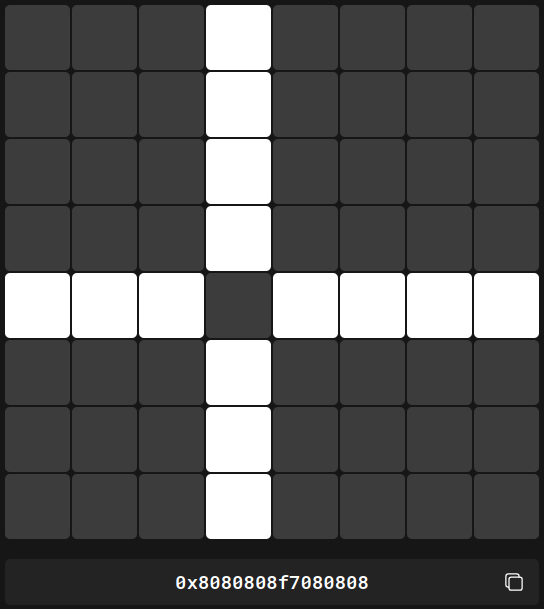
\includegraphics[width=\textwidth]{Imagenes/magics_rook_attacks.png}
        \caption*{Rook attack mask}
    \end{minipage}
    \hfill
    \begin{minipage}[c]{0.05\textwidth}
        \centering
        \Huge\texttt{->}
    \end{minipage}
    \hfill
    \begin{minipage}[c]{0.3\textwidth}
        \centering
        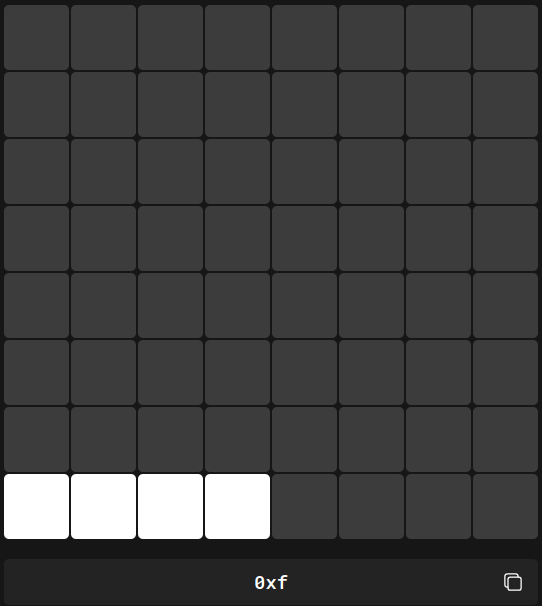
\includegraphics[width=\textwidth]{Imagenes/pext_final_index.png}
        \caption*{Final extracted index}
    \end{minipage}
    \caption{index extraction with Pext example}
    \label{fig:pext_bitboards}
\end{figure}

\noindent The final index used to access the lookup table is calculated using the \texttt{pext} instruction as follows:

\begin{align*}
    \text{index}
    &= \texttt{\_pext\_u64}(\texttt{blockers},\,\texttt{attack\_pattern})\,.
\end{align*}

\noindent To maintain compatibility and performance across different hardware platforms, we provide two implementations:

\begin{itemize}
  \item If \texttt{PEXT} support is detected at compile time, the engine uses it to compute the index directly.
  \item Otherwise, the engine falls back to the Magic Bitboards approach using multiplication and bit shifts.
\end{itemize}

\subsubsection{Analysis}

To evaluate the improvement in the move generator, we conducted the same 
100 game match vs the basic bot version.

\begin{center}
    \begin{figure}[H]
        \centering
        \ResultBar{15cm}{0.5cm}{64}{14}{22}
        \caption{Move generator with PEXT instructions bot vs basic bot}
        \label{fig:results_pext_move_generator_bot}
    \end{figure}
\medskip
\end{center}

\noindent Huge improvement with 64 wins versus 22 losses.

\subsection{Evaluation with King Safety and piece mobility}

It is often beneficial to evaluate additional aspects of a position beyond simply counting material. We introduce the following positional evaluation parameters:

\begin{enumerate}
    \item King Shield Bonus: The king is typically safer when protected by friendly pawns in front of it. We assign a bonus in the evaluation score for each allied pawn positioned directly in front of the king.

    \item King Safety Penalty: For each square within a $3 \times 3$ area surrounding the king that is attacked by enemy pieces, we apply a penalty to reflect increased vulnerability.

    \item Piece Mobility: Greater piece mobility is generally indicative of a stronger position. Each piece receives a bonus for every available move to a square that is not attacked by enemy pawns.
\end{enumerate}

\subsubsection{Analysis}

To evaluate the improvement in the new evaluation, we conducted the same 100 game match vs the basic bot version.

\vspace{1em}

\begin{center}
    \begin{figure}[H]
        \centering
        \ResultBar{15cm}{0.5cm}{62}{8}{30}
        \caption{King Safety and Piece mobility evaluation bot vs basic bot}
        \label{fig:results_safety_mobility_bot}
    \end{figure}
\medskip
\end{center}

\noindent The results are slightly worse compared to the match using the material-only evaluation,~\ref{fig:results_pext_move_generator_bot} with 8 more losses than before. This may be due to the increased computational cost of evaluating these additional parameters. Furthermore, although these are abstract concepts commonly used by humans to assess positions, the engine may struggle to find a clear correlation between them and actual positional strength.

\subsection{Search Multithread}

This version of search follows YBWC mentioned in Section~\ref{sec:alphabetaEnhancements}. It searches the first move sequentially after ordering the moves and launches the remaining moves in parallel using a thread. If it turns out that the first move was the best and pruning was applied, directly return the final node evaluation without the additional thread.

\begin{lstlisting}[breaklines=true, frame=single]
template<SearchType searchType>
static int alpha_beta_search(std::atomic<bool>& stop, int depth, int ply, int alpha, int beta, SearchContext& context, Board board)
{
    // ...
    // Check if it is in transposition table
    // If it is, return previously calculated evaluation

    generate_legal_moves<ALL_MOVES>(moves, board, &isCheck);
    // ...
    order_moves(moves, board, ply);
    // ...
    
    constexpr SearchType nextSearchType = MAXIMIZING_WHITE ? MINIMIZE_BLACK : MAXIMIZE_WHITE;

    // Search the first move sequentially
    board.make_move(moves[0]);
    int eval = alpha_beta_search<nextSearchType>(stop, depth - 1, ply + 1, alpha, beta, context, board);
    board.unmake_move(moves[0], game_state);
    // ...

    // Alpha-Beta pruning with first move
    if (/*prunned*/) goto end_search;

    // Search remaining moves in parallel
    thread = std::thread([&]() {
        for (int i = 1; i < moves.size(); i++) {
            // ...
            // Alpha-Beta pruning with the remaining moves
            if (/*prunned*/) break;
        }
    });
    
    if (thread.joinable()) {
        thread.join();
    }

end_search:
    // Store entry in tranposition table

    return final_node_evaluation;
}
\end{lstlisting}

\subsubsection{Analysis}

To evaluate the improvement in the new evaluation, we conducted the same 100 game match vs the basic bot version. 

\begin{center}
    \begin{figure}[H]
        \centering
        \ResultBar{15cm}{0.5cm}{32}{5}{63}
        \caption{Multithread Search bot vs basic bot}
        \label{fig:results_multithread_search_bot}
    \end{figure}
\medskip
\end{center}

\noindent The results are slightly worse compared to the match using the material-only evaluation, with 8 more losses than before. This may be due to the increased computational cost of evaluating these additional parameters. Furthermore, although these are abstract concepts commonly used by humans to assess positions, the engine may struggle to find a clear correlation between them and actual positional strength.

\subsection{Late Move Reductions}

We experiment with the use of late move pruning, under the assumption that if our move ordering is good, the best move in the position should be among the first explored moves. We reduce the depth by one unit starting from the tenth movement.

\subsubsection{Analysis}

To evaluate the improvement in the new evaluation, we conducted the same 100 game match vs the basic bot version.

\begin{center}
    \begin{figure}[H]
        \centering
        \ResultBar{15cm}{0.5cm}{48}{15}{37}
        \caption{Reductions Search bot vs basic bot}
        \label{fig:results_reductions_search_bot}
    \end{figure}
\medskip
\end{center}

\noindent The results are worse, with 15 more losses than the version without this aggresive pruning.~\ref{fig:results_pext_move_generator_bot} This could be because our move ordering is not that strong, and the best move in the position sometimes is in the last positions.

\section{Additional tools and work}
\label{sec:tools}

As it was mentioned in Section~\ref{sec:how}, some additional work apart from the engine implementation was done to ensure quality of the final product. This section includes some important specifications and features for the interactive board visualizer and testing worflow.

\subsection{Interactive board visualizer using CustomTkinter}

The board is implemented as a grid of squares, with each square capable of displaying a piece image. Piece images are loaded dynamically from the \texttt{assets} directory, which contains PNG files for each piece.

\vspace{1em}

\noindent The visualizer employs an event-driven architecture, where user actions, such as clicks, trigger events handled by the \texttt{EventManager} class. When the Python script is executed, it ensures that an instance of the engine in release version executable exists, starts a new subprocess with the engine, and launches a window displaying the chessboard and interface.

\begin{figure}[H]
    \centering
    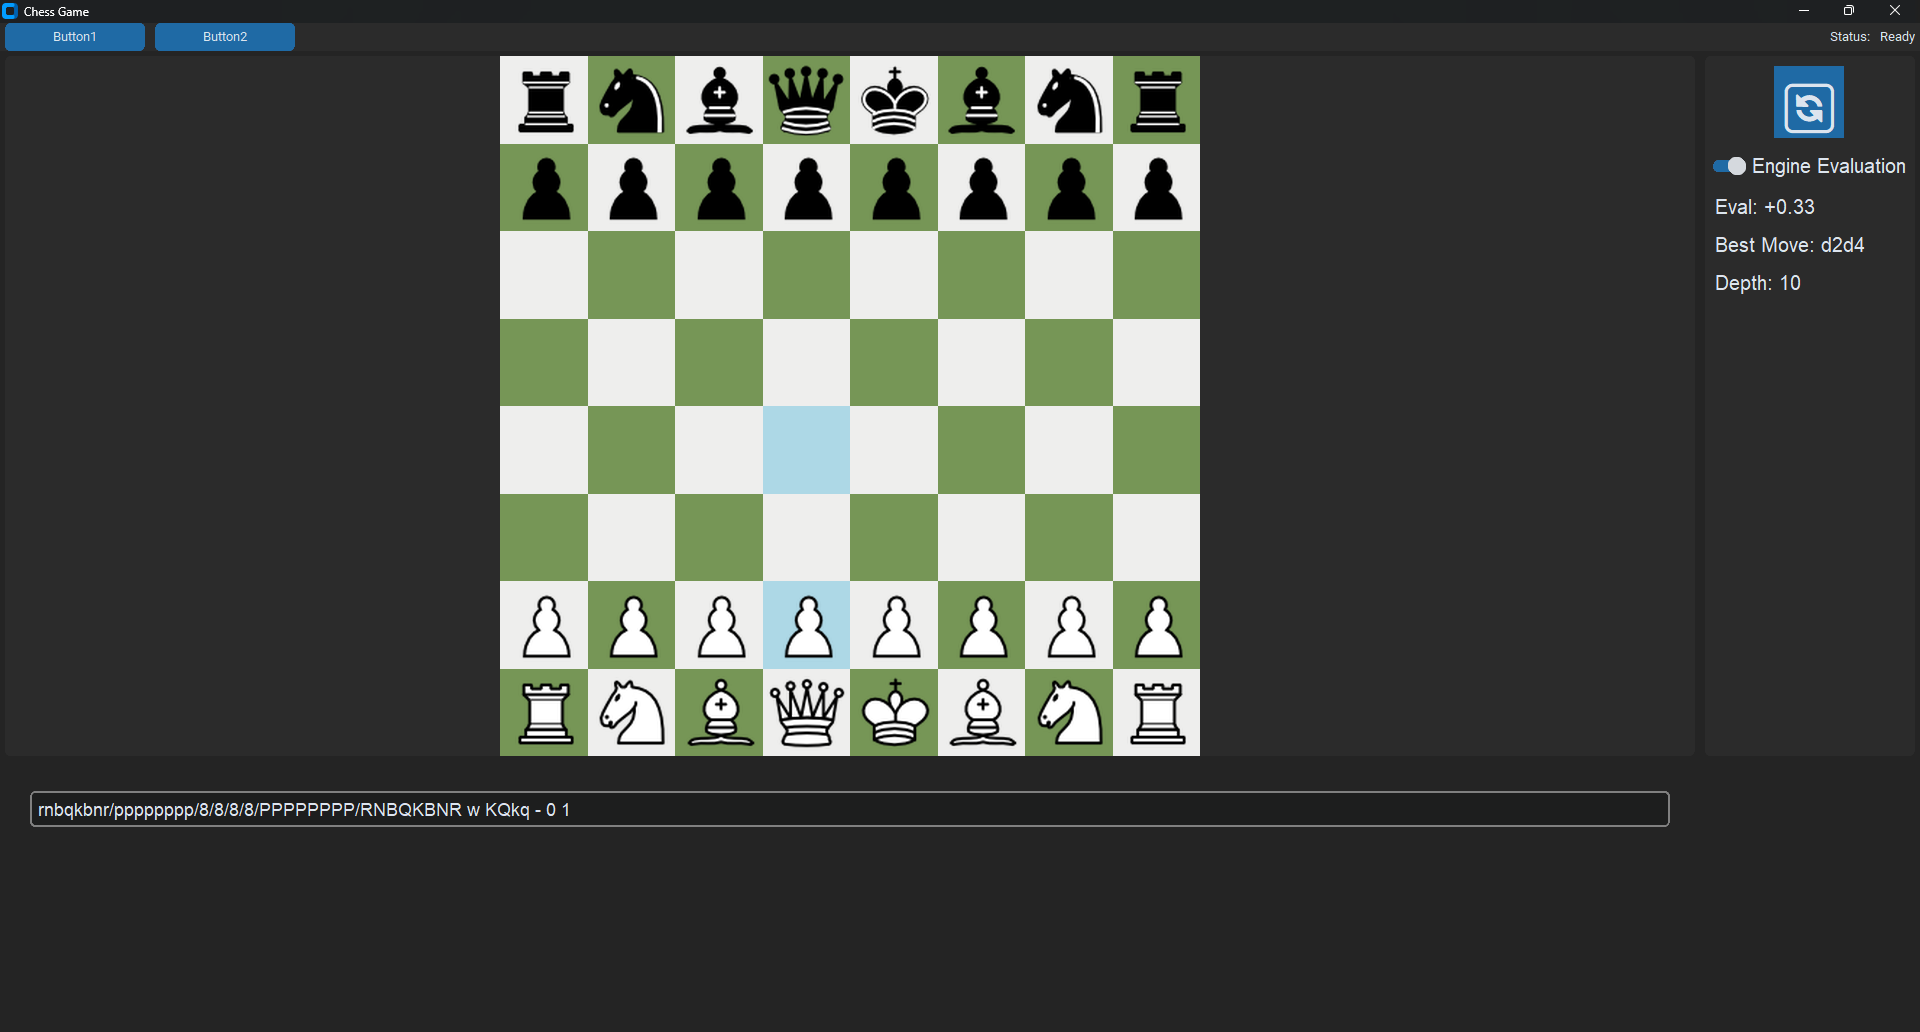
\includegraphics[width=\textwidth]{Imagenes/gui.png}
    \caption{AlphaDeepChess GUI}
    \label{fig:gui}
\end{figure}

On the right panel, there is a switch button to activate and deactivate the evaluation and suggested move in an specific depth. Also, current position's fen on the bottom panel can be modified by exchanging it to a new one.

\subsection{Testing engine strength with Cutechess, Stockfish, and GitHub Actions}

Cutechess and Stockfish can be downloaded from their respective webpages. Then, a JSON file must be provided to Cutechess to configure the available engines. An example of this \texttt{engines.json} file could be:

\vspace{1em}

\begin{lstlisting}[breaklines=true, frame=single]
[
    {
        "name": "AlphaDeepChess",
        "command": "../build/release/AlphaDeepChess",
        "protocol": "uci",
        "options": {}
    },
    {
        "name": "Stockfish",
        "command": "./stockfish/stockfish/stockfish-windows-x86-64",
        "protocol": "uci",
        "options": {
            "UCI_LimitStrength": "true",
            "UCI_Elo": "1500"
        }
    }
]
\end{lstlisting}

\noindent By simply calling the Cutechess CLI with the names of the engines and additional specifications such as search time (\texttt{--st}), the number of games (\texttt{--games}), or depth (\texttt{--depth}), the matches can be executed.

\vspace{1em}

\noindent Finally, automating this process of selecting the versions of the engine and Stockfish we created a workflow using a YAML file.

\vspace{1em}

\noindent This workflow is triggered manually. It includes the following steps:

\begin{itemize}
    \item Setup environment: Install dependencies such as Python packages, Cutechess and Stockfish.
    \item Build the engine: Compile the chess engine from source code.
    \item Run tests: Execute previously designed tests to validate the functionality of the engine using Cutechess CLI.
    \item Export generated data from Cutechess for later analysis.
\end{itemize}

This generated data are the results of the run games that includes:

\begin{itemize}
    \item A \texttt{results.epd} with all the final positions in FEN format.
    \item A \texttt{results.log} with Cutechess additional detailed information like the beginning and end of a game, the summary of the game, and ELO stadistics.
    \item A \texttt{results.pgn} with all the played moves and games.
\end{itemize}
